\documentclass[tikz, margin=25mm]{standalone}
\usepackage{tikz}
\usetikzlibrary{shapes.geometric, arrows, positioning, decorations.pathreplacing, calc, matrix, fit}
\usepackage[margin=0.5cm]{geometry}


\begin{document}

\begin{tikzpicture}[node distance=2cm and 2cm,
  % every node/.style={inner sep=0,outer sep=0}
  inner/.style={circle,draw=blue!50,fill=blue!20,thick},
  outer/.style={draw=black,fill=gray!10,thick,inner sep=10pt},
  mymatrix/.style={matrix of nodes, nodes=typetag, row sep=1em},
  mycontainer/.style={draw=gray, inner sep=1ex},
  typetag/.style={draw=gray, inner sep=1ex, anchor=west},
  title/.style={draw=none, color=gray, inner sep=0pt},
  ]

  \node[outer, remember picture] (input) {
    \begin{tikzpicture}
    \foreach \x in {1,...,4}
    {
      \node[yslant=0.5] (wsi\x) at (\x*.4,0) {
        \includegraphics[width=1.5cm, height=1.5cm]{./wsi\x.png}
      };
    }
  % Calculate the coordinates for the box
  \path (wsi1.south west) ++(0,-0.1) coordinate (bottom left);
  \path (wsi4.north east) ++(0,0.1) coordinate (top right);

  % Draw the box around the images
  \draw[black, thick] (bottom left) rectangle (top right);
  \node[below left=0.0cm and 0.9cm of bottom left, anchor=north west, text width=4.2cm, align=center] (label) {Training Data, labelled by sensitive variables };

  \end{tikzpicture}
};


\coordinate [right=3cm of input] (Model) {};
  \node[outer, remember picture] (training) at (Model) {
    \begin{tikzpicture}
\def\numLayers{5}
\def\offset{0.2}
\foreach \n in {1,...,\numLayers}
{
    \pgfmathsetmacro{\shiftX}{(\numLayers - \n) * \offset}
    \pgfmathsetmacro{\shiftY}{(\numLayers - \n) * \offset / 2}

    \draw[fill=blue!30, opacity=0.9] ([shift={(\shiftX, \shiftY)}]Model) rectangle ++(.4,-2);
}

      \node at ([shift={(2.9*\offset, -\numLayers*\offset - 1.5)}]Model) (ssl) {SSL Model};
\end{tikzpicture}
  };

\node[outer, remember picture, right=3cm of Model] (additional) {
    \begin{tikzpicture}

      \node[] (lay1) {
        \begin{tikzpicture}
\foreach \y in {0,1,...,8}
    {
        \node[circle, draw=black, fill=green, minimum size=0.01cm, scale=.3] (dot1\y) at (0, -\y*0.5) {};
    }
          \end{tikzpicture}
        };
      \node[right=-0.10cm of lay1] (lay2) {
        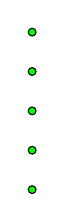
\begin{tikzpicture}
\foreach \y in {0,1,...,4}
    {
        \node[circle, draw=black, fill=green, minimum size=0.01cm, scale=.3] (dot2\y) at (0, -\y*0.5) {};
    }
          \end{tikzpicture}
        };
      \node[right=-0.10cm of lay2] (lay3) {
        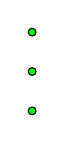
\begin{tikzpicture}
\foreach \y in {0,1,...,2}
    {
        \node[circle, draw=black, fill=green, minimum size=0.01cm, scale=.3] (dot3\y) at (0, -\y*0.5) {};
    }
          \end{tikzpicture}
        };


        \foreach \y in {0,1,...,8}
        {
            \foreach \z in {0,1,...,4}
            {
                \draw[-] (dot1\y) -- (dot2\z);
            }
        }
        \foreach \z in {0,1,...,4}
        {
          \foreach \zi in {0,1,...,2}
          {
                \draw[-] (dot2\z) -- (dot3\zi);
          }
        }

      % \node [below=.0cm of mapper] (ssl) {Additional layers};

    \end{tikzpicture}
  };

\node[outer, remember picture, below=3cm of additional] (sndTraining) {
    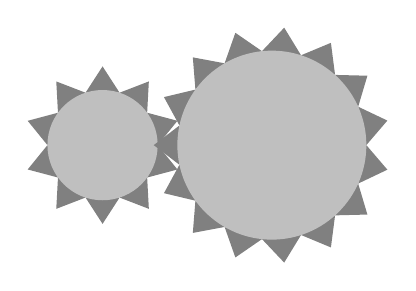
\begin{tikzpicture}
    % Parameters for the first gear
    \def\Rone{1}
    \def\rone{0.7}
    \def\teethone{10}

    % Parameters for the second gear
    \def\Rtwo{1.5}
    \def\rtwo{1.2}
    \def\teethtwo{15}
    \def\shift{2.15}

    % First gear (smaller)
    \begin{scope}
        \foreach \i in {1,...,\teethone} {
            \fill[gray] ({360/\teethone * (\i - 1)}:\rone) -- 
                        ({360/\teethone * (\i - 1) + 360/(2*\teethone)}:\Rone) -- 
                        ({360/\teethone * \i}:\rone) -- cycle;
        }
        \fill[gray!50] circle (\rone);
        % \draw[thick] circle (\rone);
    \end{scope}
    
    % Second gear (larger)
    \begin{scope}[xshift=\shift cm]
        \foreach \i in {1,...,\teethtwo} {
            \fill[gray] ({360/\teethtwo * (\i - 1)}:\rtwo) -- 
                        ({360/\teethtwo * (\i - 1) + 360/(2*\teethtwo)}:\Rtwo) -- 
                        ({360/\teethtwo * \i}:\rtwo) -- cycle;
        }
        \fill[gray!50] circle (\rtwo);
        % \draw[thick] circle (\rtwo);
    \end{scope}
\end{tikzpicture}
  };
\node[outer, remember picture, left=3cm of sndTraining] (analysis) {
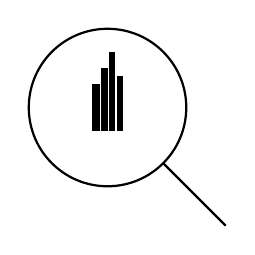
\begin{tikzpicture}
    \draw[thick] (0,0) circle (1cm); % Outer circle
    \draw[thick] (1.5,-1.5) -- (0.7,-0.7); % Handle

    \fill (-0.2,-0.3) rectangle (-0.1,0.3); % First bar
    \fill (-0.08,-0.3) rectangle (-0.0,0.5); % Second bar
    \fill (0.02,-0.3) rectangle (0.1,0.7); % Third bar
    \fill (0.12,-0.3) rectangle (0.2,0.4); % Fourth bar
\end{tikzpicture}
};

\node [above=.0cm of input] (inputText) {1. Organize input};
\node [above=.0cm of training, text width=4.0cm] (trainingText) {2. Freeze model to prevent updates};
\node [above=.0cm of additional, text width=4.0cm] (additionalText) {3. Attach additional layers to end of model};
\node [above=.0cm of sndTraining, text width=4.2cm] (retrainingText) {4. Train model with layers};
\node [above=.0cm of analysis, text width=4.2cm] (analysisText) {5. Run new model on test data, analyze results};

\draw[->] (input) -- (training);
\draw[->] (training) -- (additional);
% \draw[->] (rwsi33.south) -- ++(0,-1cm) |- ($(Model) + (1.5cm, 0)$) -- (Model);
\draw[->] (additional.east) -- ++(2.0cm,0) |- ($(sndTraining.center) + (3.0cm, 0)$);
\draw[->] (sndTraining) -- (analysis);
 
 
\end{tikzpicture}
\end{document}

